\subsection{Camera, LiDAR, and FCU}\label{subsection:D}
% TODO: add a section for lidar

First, the implementation of the Robot Operating System (ROS) on the Jetson Orin Nano involved a detailed process of hardware and software setup. This setup was fundamental for installing ROS libraries and configuring the operating system to support the demands of real-time robotic control. A key aspect of this implementation was the development of custom ROS nodes. These nodes were designed to perform specific functions such as data acquisition, processing, and transmission of commands. They were capable of publishing and subscribing to topics within the ROS environment, facilitating a dynamic data exchange system.

Next, various sensors were integrated, including cameras, GPS, IMUs, and LiDAR into the ROS framework, this required the development of custom drivers and interfaces to ensure a seamless flow of data from the sensors into the ROS system. In parallel, a robust connection between the Jetson Orin Nano and the drone's flight control unit was established using MAVROS and MAVProxy. MAVROS acted as a bridge, enabling real-time communication and command exchange. A link with this protocol was set up for transmitting control commands from the ROS nodes to the drone and for receiving flight data from various sensors in the flight control unit.

Then, to enhance the drone's sensory capabilities, the drone involved mounting additional cameras and LiDAR \cite{2d1}, as shown in Fig. ~\ref{fig2d1}. The placement of these sensors was strategically chosen to optimize the field of view and depth perception. An important step in this process was the calibration of the sensors to ensure accuracy in data capture. Algorithms were then developed to merge data streams from these cameras and Lidar. This fusion created a comprehensive view combining both image and depth information, essential for advanced perception. To ensure efficiency, the optimized image capture package V4L was employed instead of openCV to minimize latency in data transfer and processing. RVIZ, a visualization tool within ROS, was customized for real-time monitoring and debugging of the fused data. This setup facilitated a clear visualization of how image and depth data were combined, aiding in system refinement and development.
    \begin{figure}[H]
        \centerline{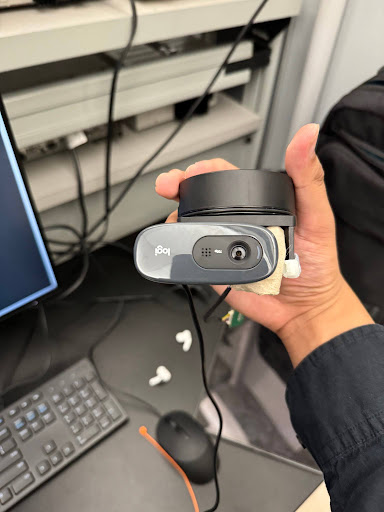
\includegraphics[width=0.3\textwidth]{Figures/Methods/physical_setup.jpg}}
        \caption{Physical Setup of the Camera and Lidar}
        \label{fig2d1}
    \end{figure}
The project focused on developing algorithms for obstacle avoidance, tracking, person detection, and counting. These algorithms were designed to utilize the data provided by the integrated sensors, enabling the drone to dynamically interact with its environment. Gazebo, a robotic simulator was heavily used in testing these algorithms, as shown in Fig. ~\ref{fig2d2}. It provided a controlled environment to simulate various scenarios, allowing for the fine-tuning of algorithms before real-world application. By setting up the obstacles in the simulated world, the drone's obstacle avoidance function can be tested by letting the drone found its own way out in a maze. This process involved the use of Lidar and the motion control of the drone.

    \begin{figure}[H]
        \centerline{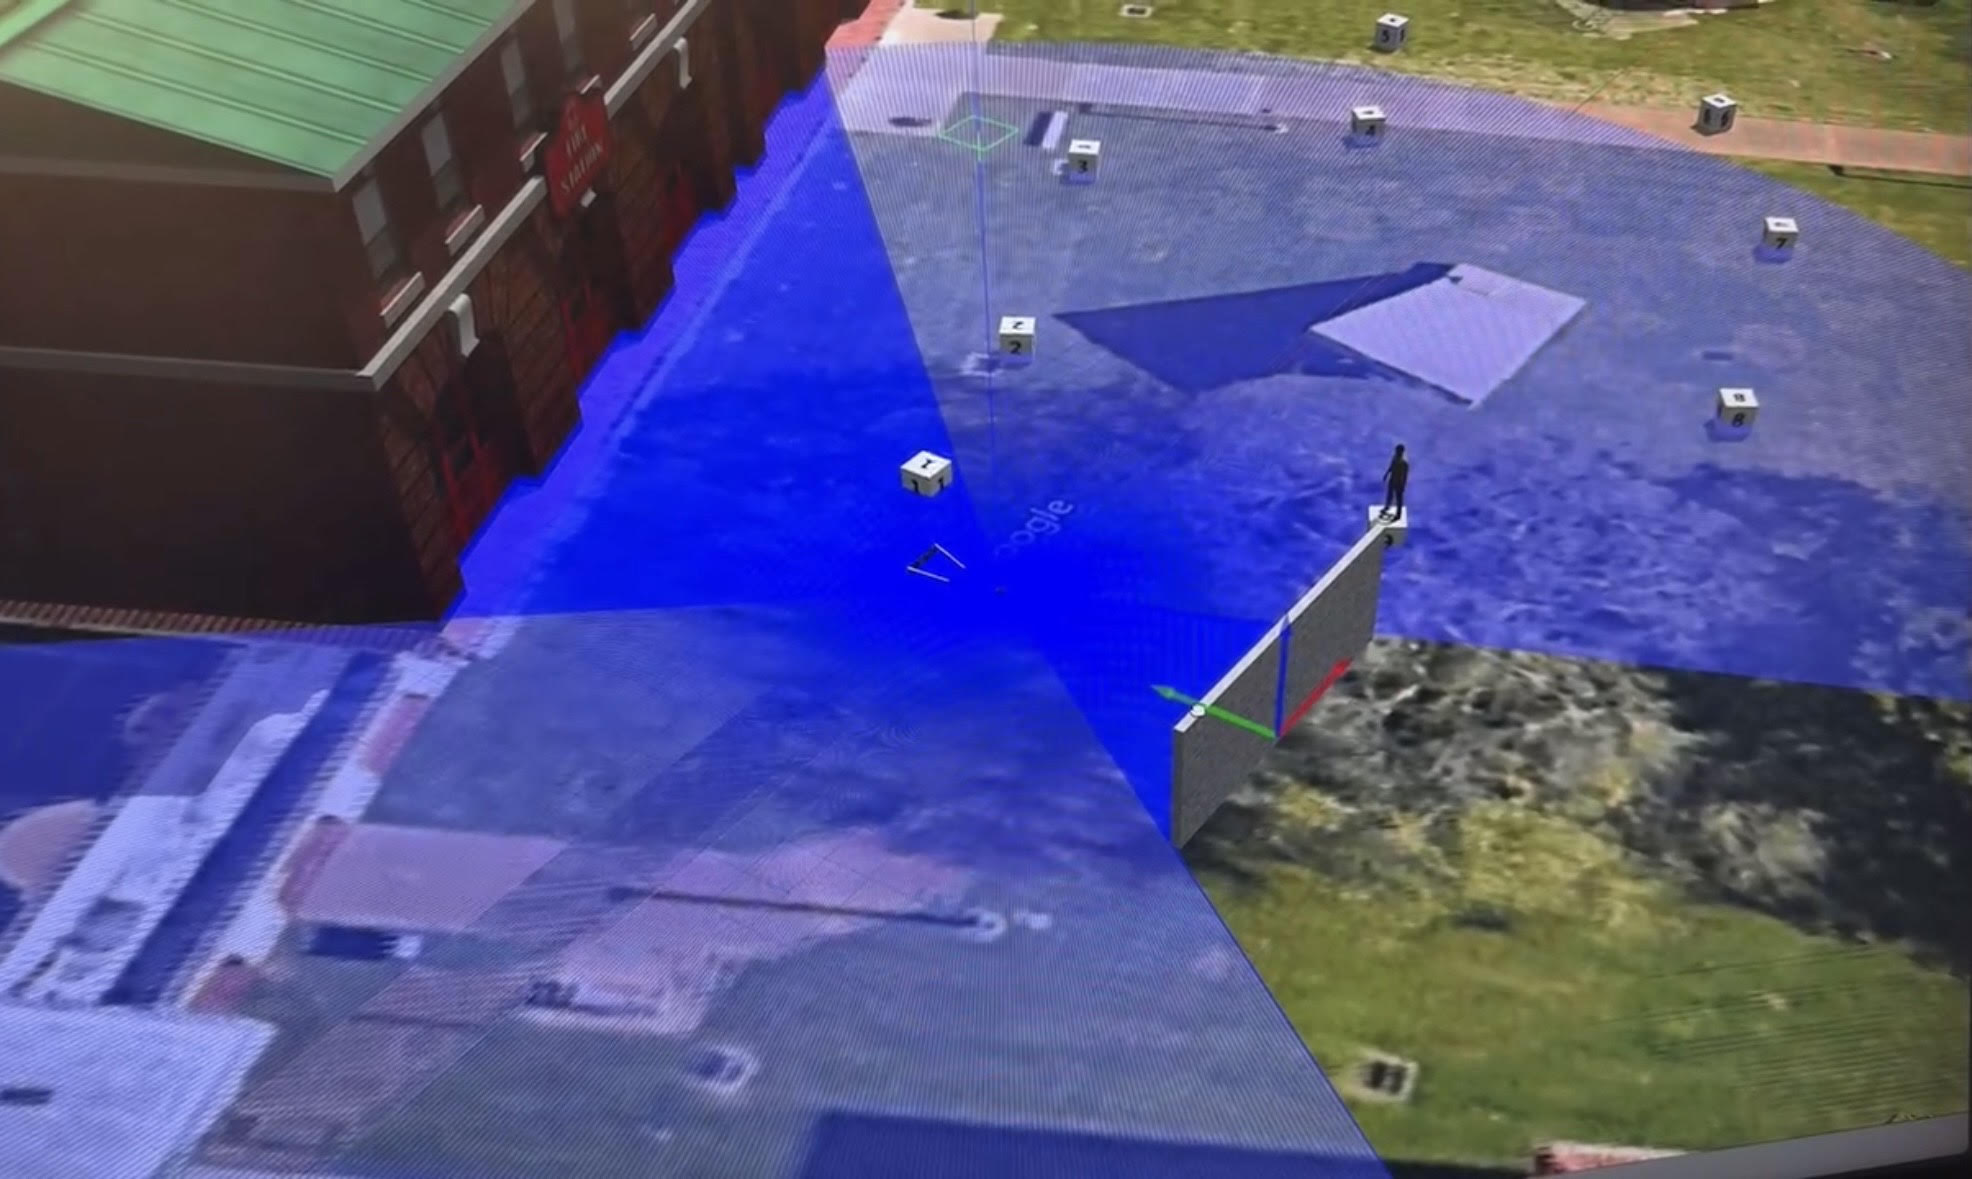
\includegraphics[width=0.5\textwidth]{Figures/Methods/gazebo_lidar.jpg}}
        \caption{Scenario Setup in Gazebo}
        \label{fig2d2}
    \end{figure}
    
Finally, the data collection and analysis during these simulations were vital in assessing and optimizing the performance of the algorithms. This iterative process involved making adjustments based on performance metrics to enhance efficiency and accuracy. Once the algorithms were satisfactorily developed and tested in the simulator, they were integrated into the ROS environment. This integration entailed coding the algorithms into ROS nodes and ensuring they interacted seamlessly with other system components. Preliminary field tests were then conducted to evaluate the performance of these algorithms in real-world conditions, with observations from these tests used to make further adjustments and improvements.
